%% Template for MLP Coursework 2 / 6 November 2017 

%% Based on  LaTeX template for ICML 2017 - example_paper.tex at 
%%  https://2017.icml.cc/Conferences/2017/StyleAuthorInstructions

\documentclass{article}

\usepackage[T1]{fontenc}
\usepackage{amssymb,amsmath}
\usepackage{txfonts}
\usepackage{microtype}
\usepackage{float}

% For figures
\usepackage{graphicx}
\usepackage{subfigure} 

% For citations
\usepackage{natbib}

% For algorithms
\usepackage{algorithm}
\usepackage{algorithmic}

% the hyperref package is used to produce hyperlinks in the
% resulting PDF.  If this breaks your system, please commend out the
% following usepackage line and replace \usepackage{mlp2017} with
% \usepackage[nohyperref]{mlp2017} below.
\usepackage{hyperref}
\usepackage{url}
\urlstyle{same}

% Packages hyperref and algorithmic misbehave sometimes.  We can fix
% this with the following command.
\newcommand{\theHalgorithm}{\arabic{algorithm}}


% Set up MLP coursework style (based on ICML style)
\usepackage{mlp2017}
\mlptitlerunning{MLP Coursework 2 (\studentNumber)}
\bibliographystyle{icml2017}


\DeclareMathOperator{\softmax}{softmax}
\DeclareMathOperator{\sigmoid}{sigmoid}
\DeclareMathOperator{\sgn}{sgn}
\DeclareMathOperator{\relu}{relu}
\DeclareMathOperator{\lrelu}{lrelu}
\DeclareMathOperator{\elu}{elu}
\DeclareMathOperator{\selu}{selu}
\DeclareMathOperator{\maxout}{maxout}

%% You probably do not need to change anything above this comment

%% REPLACE this with your student number
\def\studentNumber{s1679450}

\begin{document} 

\twocolumn[
\mlptitle{MLP Coursework 2: Learning rules, BatchNorm, and ConvNets}

\centerline{\studentNumber}

\vskip 7mm
]

\begin{abstract} 
This paper focus on the classification task of EMNIST dataset. First we set up the baseline model, discussed the selection of activation function, number of hidden layer, regularization method and dropout rate. After we setup the baseline model, we start to investigate the influence of different learning rules. Then we evaluated the performance of Batch normalization layer. Finally we discussed the performance of convolutional layer and how different  convolutional layer parameters will influence the result. 
\end{abstract} 

\section{Introduction}
\label{sec:intro}
%This document provides a template for the MLP coursework 2 report.  This template structures the report into sections, which you are recommended to use, but can change if you wish.  If you want to use subsections within a section that is fine, but please do not use any deeper structuring.  In this template the text in each section will include an outline of what you should include in each section, along with some practical \LaTeX\ examples (for example figures, tables, algorithms).  Your document should be no longer than \textbf{seven pages},  with an additional page allowed for references.


%The introduction should place your work in context, giving the overall motivation for the work, and clearly outlining the research questions you have explored.  This section should also include a concise description of the Balanced EMNIST task and  data -- be precise: for example state the size of the training, validation, and test sets.

The classification problem is a important part of machine learning and handwritten letters is quite frequently used to evaluate machine learning system performances. EMNIST\citep{DBLP:journals/corr/CohenATS17} is a new dataset for handwritten letters recognition. 

We are going to explore how different mechanisms will work on EMNIST dataset. We  will first evaluate simple neural network classifier, and use the tuned result as baseline for following discussions. For different learning rules, we are going discuss about their difference and their actual performance on the dataset. Also we will try to explain the result of experiment. Secondly, we will discuss about the concept of batch normalization and in what aspect it's going to help machine learning systems. Finally, we will explain about convolutional network models and discuss about efficient ways to implement  a convolutional layer. Also, we will evaluate the performance of our convolutional layer and try to explain how the parameters of convolutional layer is going to influence the classification result.

We will train our system on a training set of 100000 examples,  evaluate the performance on validation set of 15800 examples and test the model using test set of 15800 examples.






\section{Baseline systems} 
\begin{itemize}
	\item Learning Algorithm: Stochastic gradient descent with 0.1 learning rate.
	\item Batch size: 100.
	\item Training epoch number: 50.
\end{itemize}

The hyper parameters above we won't change during this part. There are few properties we want to investigate in the following part : activation function, hidden layer number, regularization method, dropout rate.

\subsection{Activation function selection}
In this section, we compared different type of activation function to find out their performance on the EMNIST dataset.
\paragraph{Restricted Linear Unit (ReLU)}
ReLU \citep{icml2010_NairH10} has the following form.
\begin{equation}
  \relu(x) = \max(0, x) ,
\end{equation} 
which has the gradient:
\begin{equation}
  \frac{d}{dx} \relu(x) =
     \begin{cases} 
      0      & \quad \text{if } x \leq  0 \\
      1       & \quad \text{if } x > 0 .
    \end{cases} 
\end{equation}

\paragraph{Leaky Restricted Linear Unit (Leaky ReLU)}
Leaky ReLU \citep{Maas13rectifiernonlinearities} has the following form.
\begin{equation}
	\lrelu(x) = 
	\begin{cases} 
      \alpha x      & \quad \text{if } x \leq  0 \\
      x      & \quad \text{if } x > 0 .
    \end{cases} 
\end{equation}
which has the gradient:
\begin{equation}
  \frac{d}{dx} \lrelu(x) =
     \begin{cases} 
      \alpha      & \quad \text{if } x \leq  0 \\
      1       & \quad \text{if } x > 0 .
    \end{cases} 
\end{equation}

\paragraph{Exponential Linear Units (ELU)}
ELU\citep{2015arXiv151107289C} has the following form
\begin{equation}
	\elu(x) = 
	\begin{cases} 
      \alpha (\exp(x)-1)      & \quad \text{if } x \leq  0 \\
      x      & \quad \text{if } x > 0 .
    \end{cases} 
\end{equation}
which has the gradient:
\begin{equation}
  \frac{d}{dx} \elu(x) =
     \begin{cases} 
      \alpha \exp(x)     & \quad \text{if } x \leq  0 \\
      1       & \quad \text{if } x > 0 .
    \end{cases} 
\end{equation}


\paragraph{Scaled Exponential Linear Units (SELU)}
SELU \citep{2017arXiv170602515K} has the following form.
\begin{equation}
	\selu(x) = \lambda
	\begin{cases} 
      \alpha (\exp(x)-1)      & \quad \text{if } x \leq  0 \\
      x      & \quad \text{if } x > 0 .
    \end{cases} 
\end{equation}
which has the gradient:
\begin{equation}
  \frac{d}{dx} \elu(x) = \lambda
     \begin{cases} 
      \alpha \exp(x)     & \quad \text{if } x \leq  0 \\
      1       & \quad \text{if } x > 0 .
    \end{cases} 
\end{equation}

As Figure~\ref{fig:base_act_func} shows, ELU have the best overall performance: both in validation set and training set. ELU always has better accuracy and lower cross-entropy error than other activation functions. In test set, ELU also has best accuracy.


\begin{table}[tb]
\vskip 3mm
\begin{center}
\begin{small}
\begin{sc}
\begin{tabular}{lcccr}
\hline
\abovespace\belowspace
Activation function & Accuracy \\
\hline
\abovespace
ELU    	& 0.8270 	\\
SELU 	& 0.8189 	\\
LRELU  	& 0.8204 	\\
RELU	& 0.8186	\\

\hline
\end{tabular}
\end{sc}
\end{small}
\caption{Accuracy of models with different activation function on test set}
\label{tab:activation_func}
\end{center}
\vskip -3mm
\end{table}


\begin{figure}[tb]
\begin{center}
\centerline{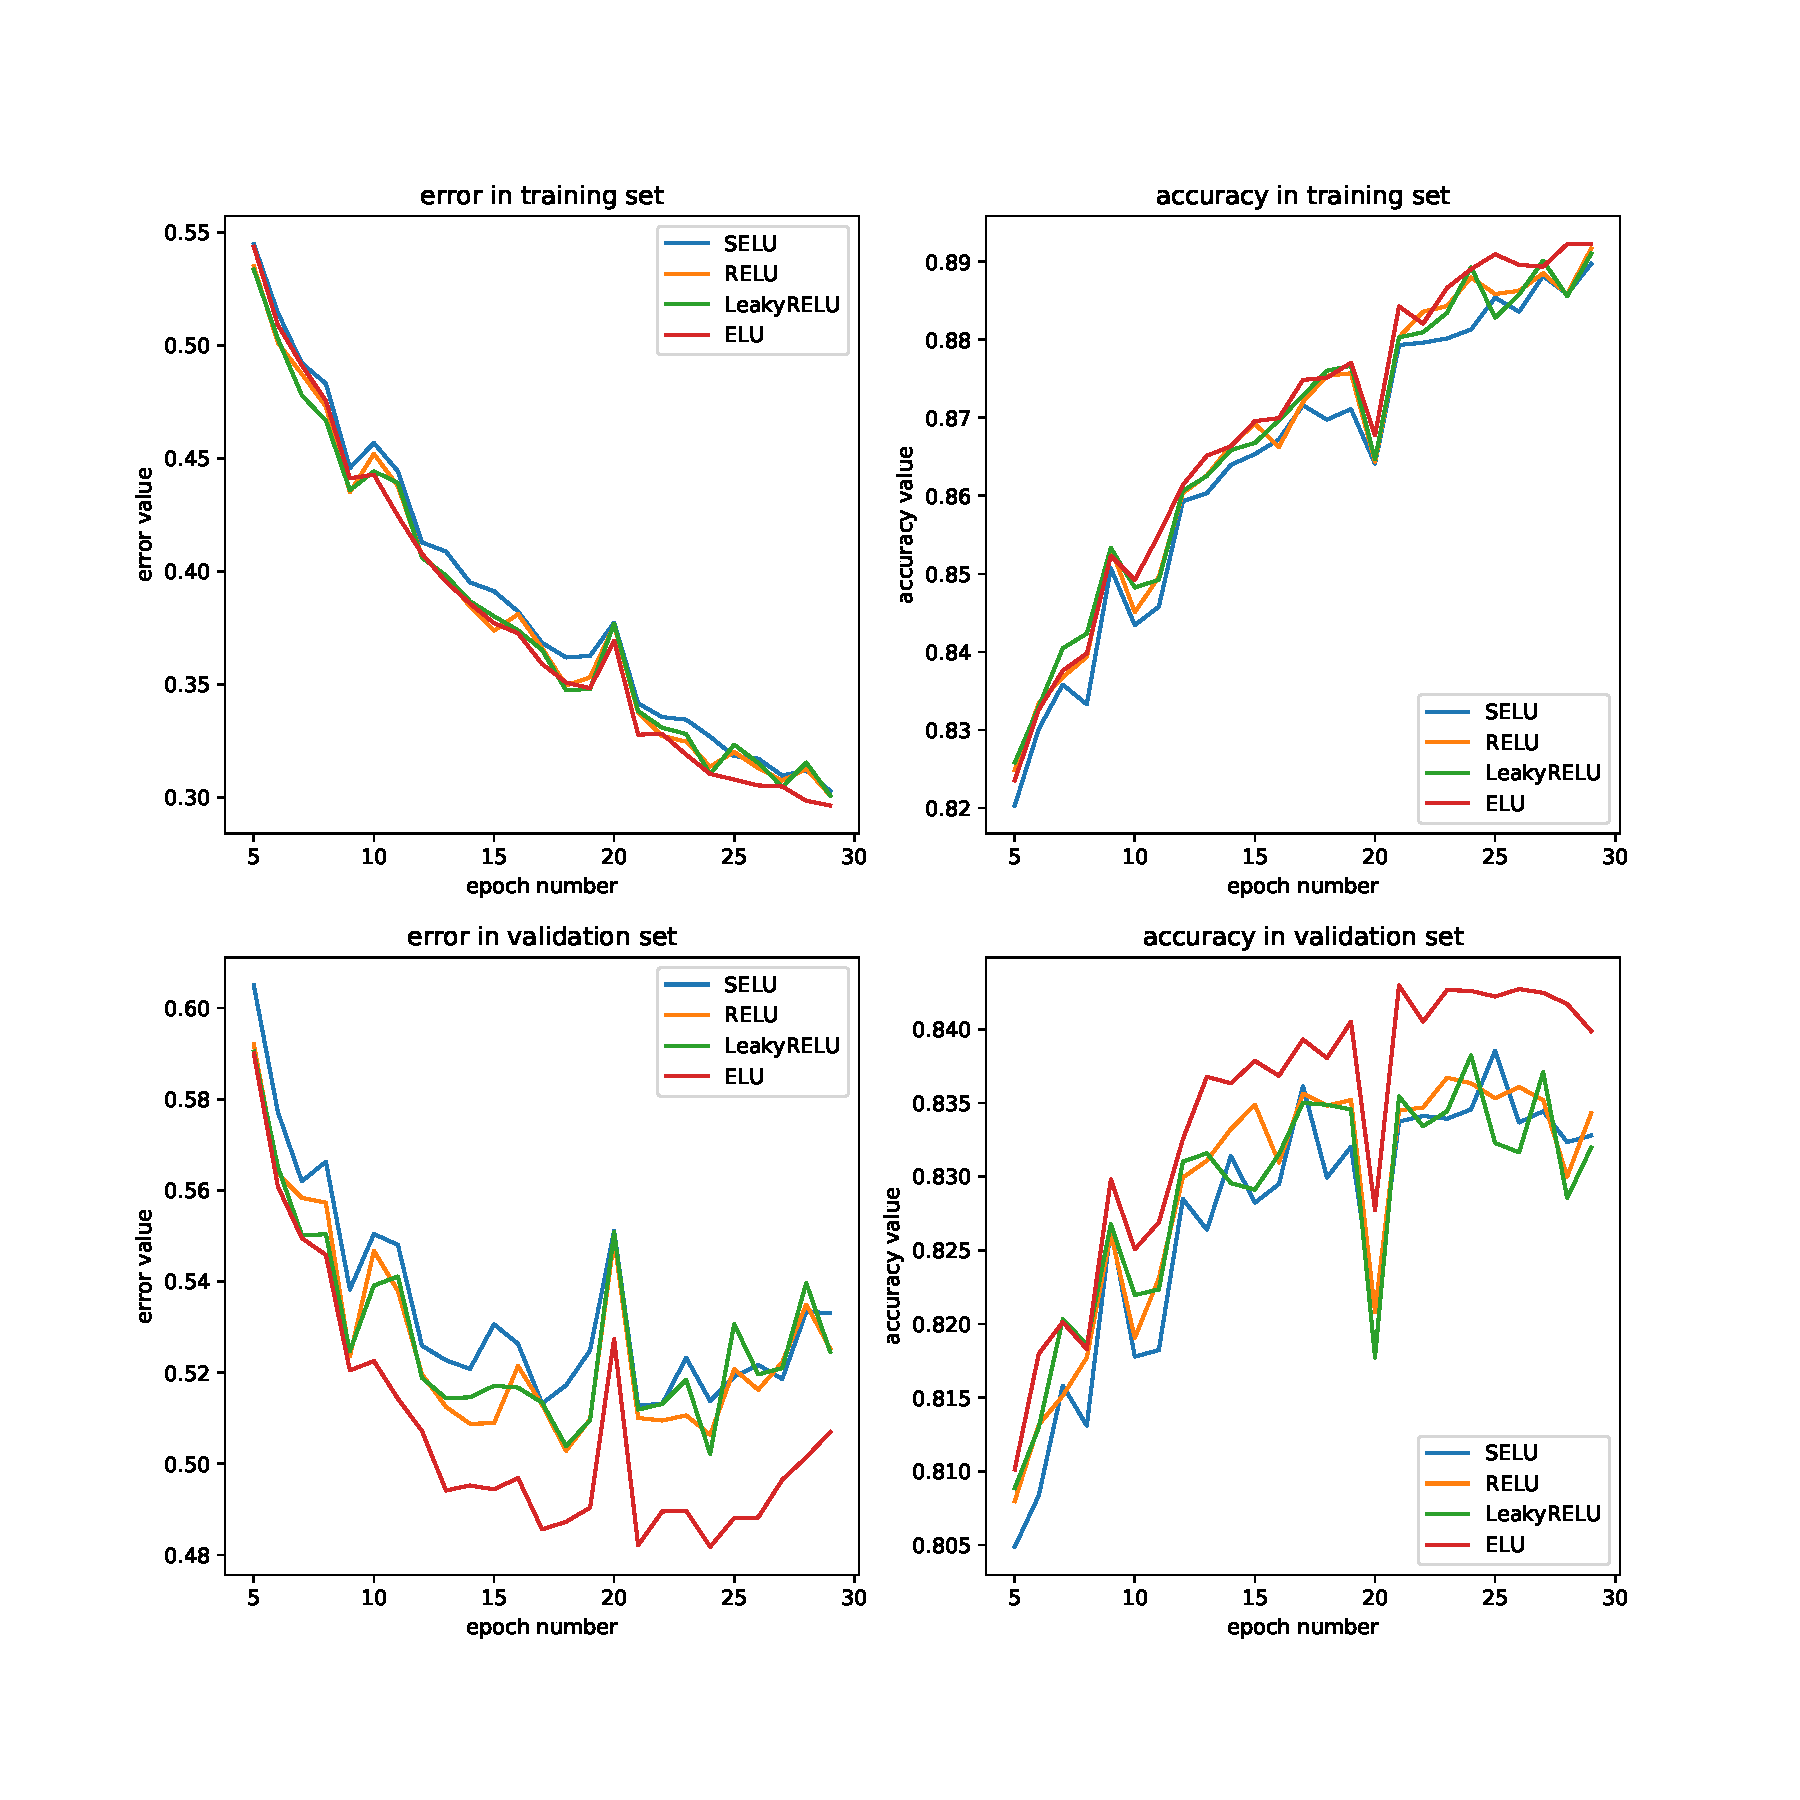
\includegraphics[width=\columnwidth]{fig/activation_function.pdf}}
\caption{Comparison between models with different kind of activation functions.}
\label{fig:base_act_func}
\end{center}
\end{figure} 


\subsection{Number of hidden layers}
 On top of the result of activation functions, we evaluated the influence of different number of hidden layers. As we know, deeper network model can learn more complex decision boundaries. Compared with MNIST dataset, the output class number of EMNIST increased from 10 to 48, which might need deeper network to draw the decision boundary. We can see from the result in Figure~\ref{fig:base_num_layer}, having deeper layer number can result in better accuracy but higher possibility to overfit. From the Table~\ref{tab:layer_num} we can see that the accuracy is getting lower. The reason is at current stage we are not applying any early stopping mechanism or use other methods to stop overfitting. So we finally choose the best overall performance one: the network with 4 hidden layer.
 

\begin{table}[tb]
\vskip 3mm
\begin{center}
\begin{small}
\begin{sc}
\begin{tabular}{lcccr}
\hline
\abovespace\belowspace
Layer number & Accuracy \\
\hline
\abovespace
2    	& 0.8270 	\\
3	 	& 0.8222 	\\
4	  	& 0.8193 	\\
% 5! %

\hline
\end{tabular}
\end{sc}
\end{small}
\caption{Accuracy of models with different hidden layer number on test set}
\label{tab:layer_num}
\end{center}
\vskip -3mm
\end{table}


\begin{figure}[tb]
\begin{center}
\centerline{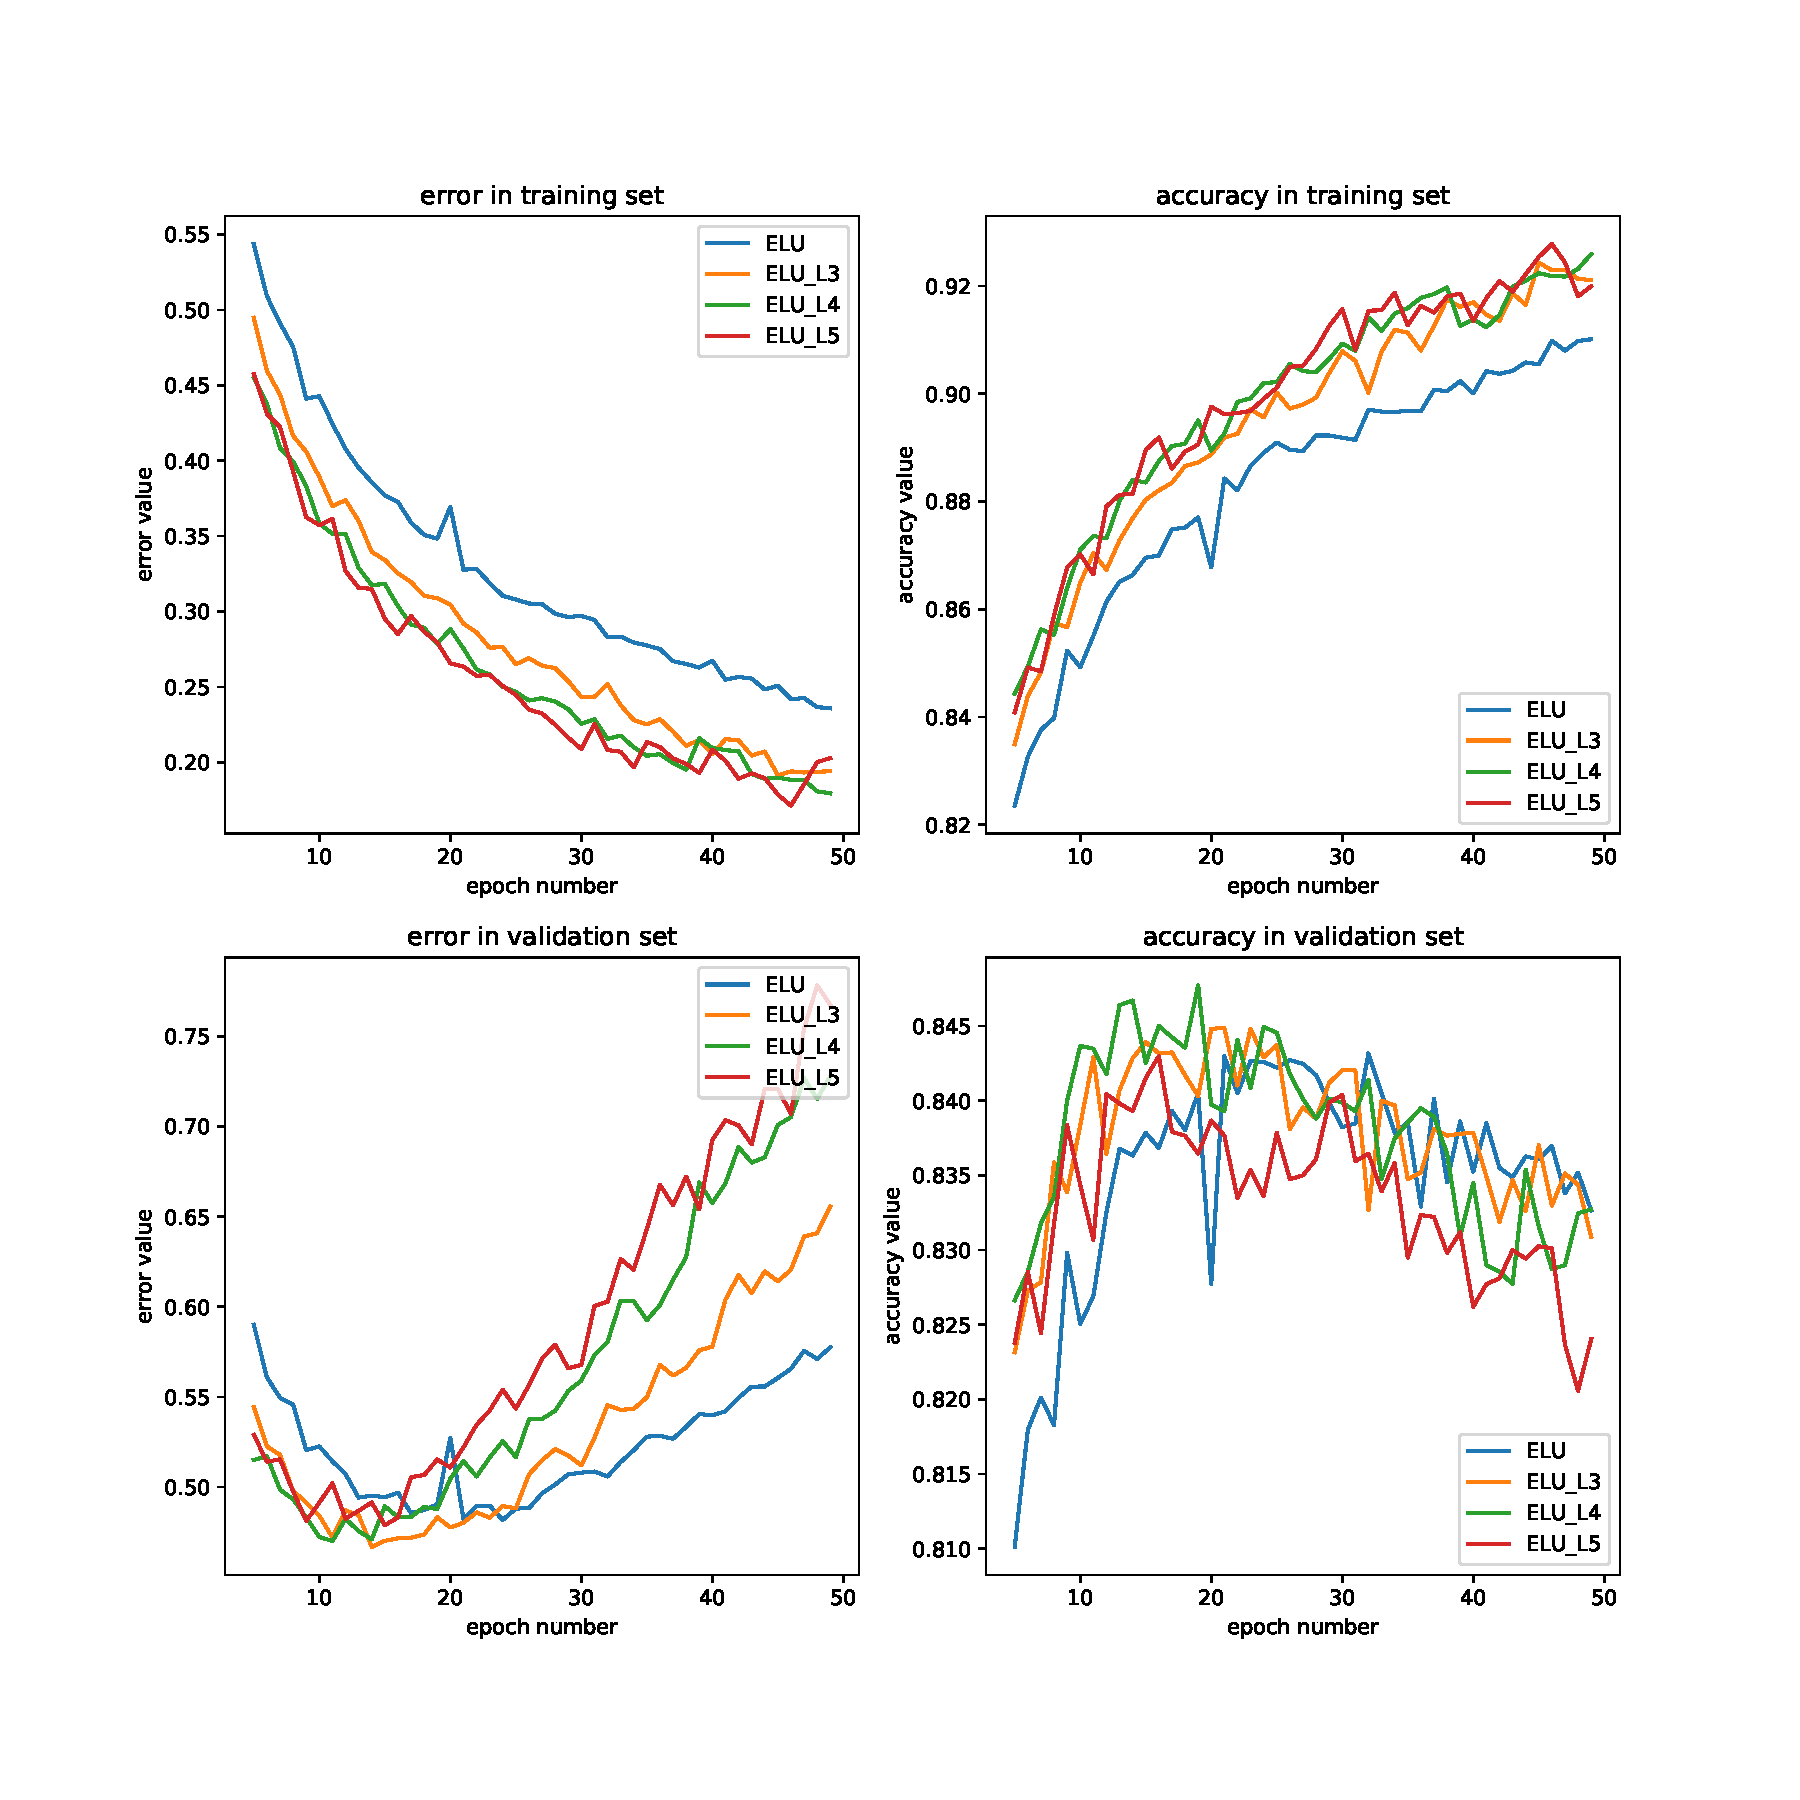
\includegraphics[width=\columnwidth]{fig/num_layer.pdf}}
\caption{Comparison between models with different number of hidden layers. }
\label{fig:base_num_layer}
\end{center}
\end{figure} 










\subsection{Regularization}
We have discussed in previous part that deeper network can have higher possibility to overfit. In order to alleviate the influence of overfitting, we are going to use regularization. 


Regularization is basically adding regularization terms to the error function. Based on regularization type, they are penalizing specific features by increasing error. L1 regularization is adding the sum of absolute values of the weights to error. L2 regularization is the sum of the squares of all the weights in the network and then multiplied by $\frac{\lambda}{2n}$. Both of these regularization methods will penalize big weights. % L1 and L2 specified penalize thing%


The result is in Figure~\ref{fig:base_reg}. In the error distribution, we can see that if regularization parameter is not small enough, then it will cause the error to stay in a high level and influence the final result of training.  From the curve of error in validation set, we can see that regularisation successfully suppress the increase trend of validation set error. The one with best overall performance is L2 regularization with decay rate at 1e-4 (0.0001).


\begin{table}[tb]
\vskip 3mm
\begin{center}
\begin{small}
\begin{sc}
\begin{tabular}{lcccr}
\hline
\abovespace\belowspace
Regularization Method & Accuracy \\
\hline
\abovespace
None					& 0.8193		\\
L1Penalty(1e-05)    	& 0.8247 	\\
L1Penalty(0.001)	 	& 0.7296 	\\
L2Penalty(0.0001)		& 0.8322  	\\
L2Penalty(0.01)	  		& 0.7196 	\\

% 5! %

\hline
\end{tabular}
\end{sc}
\end{small}
\caption{Accuracy of models with different regularization on test set}
\label{tab:reg}
\end{center}
\vskip -3mm
\end{table}





\begin{figure}[tb]
\begin{center}
\centerline{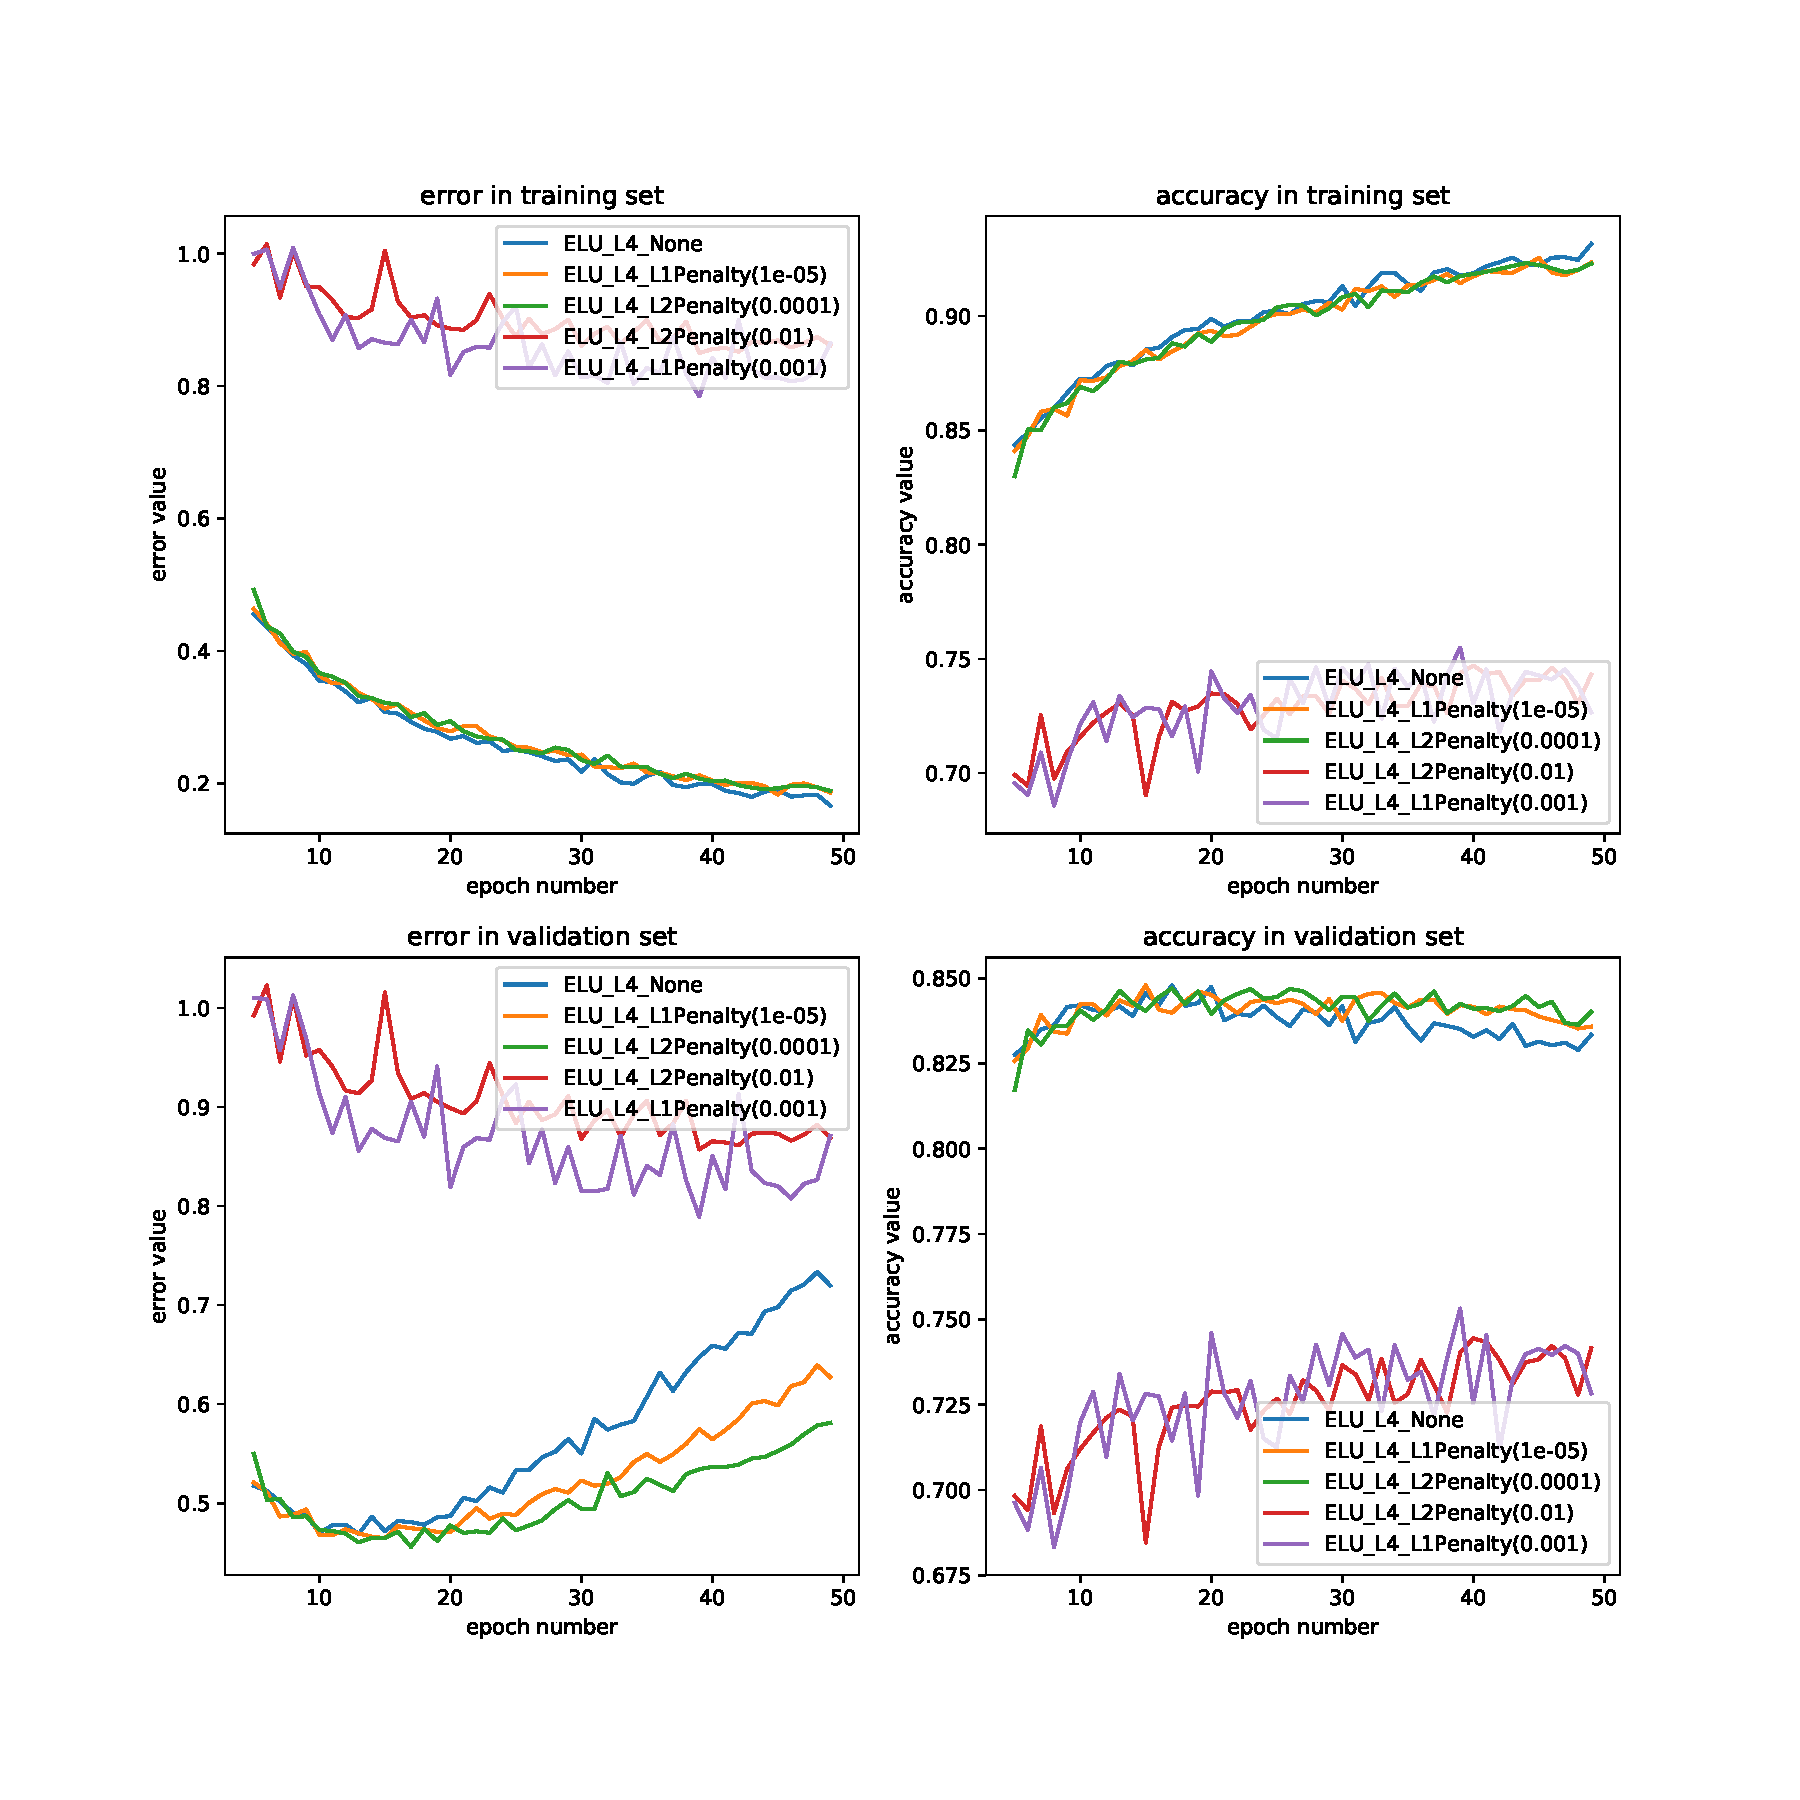
\includegraphics[width=\columnwidth]{fig/reg.pdf}}
\caption{Comparison between models with different regularization methods.}
\label{fig:base_reg}
\end{center}
\end{figure} 


\subsection{Dropout layer}

Dropout layer \citep{JMLR:v15:srivastava14a} is a simple layer which will randomly drop some of the unit and their connection to alleviate  overfitting.

Adding dropout layer is another method to alleviate overfitting issue. But higher dropout rate can result in slower training process ( i.e.  need more epoch to converge). The result is showed in Figure~\ref{fig:base_dropout}. Compared with the baseline, adding dropout layer can  significantly reduce overfitting tread. The models with dropout trains slower in training set, but unlike the one without dropout, the curve never shows a trend to overfit in validation set.  

%In this section you should  report your baseline experiments for EMNIST.  No need for theoretical explanations of things covered in the course, but should you go beyond what was covered please explain what you did with references to relevant paper(s) if appropriate.   In this section you should aim to cover the both the ``what'' and the ``why'': \emph{what} you did, giving sufficient information (hyperparameter settings, etc.) so that someone else (e.g. another student on the course) could reproduce your results; and \emph{why} you performed the experiments you are reporting - what you are aiming to discover what is the motivation for the particular experiments you undertook. You should also provide some discussion and interpretation of your results.  

% As before, your experimental sections should include graphs (for instance, figure~\ref{fig:sample-graph}) and/or tables (for instance, table~\ref{tab:sample-table})\footnote{These examples were taken from the ICML template paper.}, using the \verb+figure+ and \verb+table+ environments, in which you use \verb+\includegraphics+ to include an image (pdf, png, or jpg formats).  Please export graphs as 

\begin{table}[tb]
\vskip 3mm
\begin{center}
\begin{small}
\begin{sc}
\begin{tabular}{lcccr}
\hline
\abovespace\belowspace
Dropout percent & Accuracy \\
\hline
\abovespace
0.0    	& 0.8193 	\\
0.1 	& 0.8561 	\\
0.2  	& 0.8433 	\\
0.3		& 0.8214	\\

\hline
\end{tabular}
\end{sc}
\end{small}
\caption{Accuracy of models with different activation on test set}
\label{tab:dropout}
\end{center}
\vskip -3mm
\end{table}






\subsection{Final baseline model}
After all the discussions above, the final model we choose for baseline is
\begin{itemize}
	\item ELU activation function
	\item 4 hidden layers with 100 hidden units per layer
	\item L2 regularization (decay rate: 0.0001)
	\item Dropout layer (Drop 0.1)
\end{itemize}


 
%
%\href{https://en.wikipedia.org/wiki/Vector_graphics}{vector graphics}
%rather than \href{https://en.wikipedia.org/wiki/Raster_graphics}{raster
%files} as this will make sure all detail in the plot is visible.
%Matplotlib supports saving high quality figures in a wide range of
%common image formats using the
%\href{http://matplotlib.org/api/pyplot_api.html\#matplotlib.pyplot.savefig}{\texttt{savefig}}
%function. \textbf{You should use \texttt{savefig} rather than copying
%the screen-resolution raster images outputted in the notebook.} An
%example of using \texttt{savefig} to save a figure as a PDF file (which
%can be included as graphics in a \LaTeX document is given in the coursework 1 document.
%
%If you need a figure or table to stretch across two columns use the \verb+figure*+ or \verb+table*+ environment instead of the \verb+figure+ or \verb+table+ environment.  Use the \verb+subfigure+ environment if you want to include multiple graphics in a single figure.


\section{Learning rules}
%In this section you should compare RMSProp and Adam with gradient descent, introducing these learning rules either as equations or as algorithmic pseudocode.  If you present the different approaches as algorithms, you can use the \verb+algorithm+ and \verb+algorithmic+ environments to format pseudocode (for instance, Algorithm~\ref{alg:example}). These require the corresponding style files, \verb+algorithm.sty+ and \verb+algorithmic.sty+ which are supplied with this package. 
In this section we will evaluate the performance of different learning rules on EMNIST dataset.



\begin{algorithm}[ht]
\begin{algorithmic}
   \STATE {\bfseries Input:} step size $\alpha$, size $m$
   \STATE {\bfseries Input:} $\beta_1 , \beta_2 \in [0,1)  $: Exponential decay rates for the moment estimates
   \STATE {\bfseries Input:} $f(\theta)$: Stochastic objective function with parameters $\theta$
   \STATE {\bfseries Input:} $\theta$: Initial parameter vector
   \STATE $m_0  \gets 0$ (Initialize 1 st moment vector)
   \STATE $v_0 \gets 0$ (Initialize 2 nd moment vector)
   \STATE $t \gets 0$ (Initialize timestep)   
   \WHILE{$\theta_t$ not converge}
   \STATE $ t \gets t+1 $
   \STATE $ g_t \gets \nabla_\theta f_t ( \theta_{t-1} )  $
   \STATE $ m_t \gets \beta_1 \cdot m_{t-1} + (1-\beta_1) \cdot g_t $
   \STATE $ v_t \gets \beta_2 \cdot v_{t-1} + (1-\beta_2) \cdot g_t^2 $
   \STATE $ \hat m_t \gets  m_{t} /   (1-\beta_1^t)  $
   \STATE $ \hat v_t \gets  v_{t} /   (1-\beta_2^t)  $
   \STATE $ \theta_t \gets \theta_{t-1} - \alpha \cdot \hat m_{t} / 
   \sqrt{ \hat v_t } + \epsilon $
   \ENDWHILE
   \STATE \textbf{return} $\theta_t$
   
\end{algorithmic}
  \caption{Adam Learning Rule}
  \label{alg:adam}
\end{algorithm}


\subsection{Compare different learning rules}
The original learning rule we use is  Gradient Descent, which is simply moving the step (learning rate * gradient) in the negative gradient direction. One of the shortcomings of this method is that different weights can have different magnitude of gradients. So choosing a right global learning rate is hard. To solve these issues, we are going to use learning rules with adaptive learning rate.

\paragraph{RMSProp} RMSProp \citep{Tieleman2012} is based on RProp\citep{rprop}. RProp suggests that we can use only the sign of the gradient and move same step size. This can prevent the issue like some huge gradient suddenly appears. But RProp won't work for mini-batch. Because RProp is equivalent of using a learning rate of $ \frac{1}{g_i}$($g_i$ is the gradient) where $g_i$ can be quite different over different mini batch. Having random learning rate can make converge more difficult \citep{Tieleman2012}. RMSProp can solve the problem by setting learning rate similar to previous mini batches. 
  $$S_i(0) = 0$$
  $$S_i(t) = \beta S_i(t-1) + (1 - \beta)g_i(t)^2$$
  $$ \Delta w_i(t) = \frac{ -\eta }{ \sqrt{S_i(t)} + \epsilon } g_i(t)$$
  The equation above is how RMSProp updates weight. 
\paragraph{Adam} Adam \citep{DBLP:journals/corr/KingmaB14} is simply combining RMSProp with momentum.  The algorithm of Adam learning rule is described as Algorithm~\ref{alg:adam}.

 


\begin{table}[tb]
\vskip 3mm
\begin{center}
\begin{small}
\begin{sc}
\begin{tabular}{lcccr}
\hline
\abovespace\belowspace
Learning rule & Accuracy \\
\hline
\abovespace
Adam    	& 0.8491 	\\
RMSProp	 	& 0.8508 	\\
SGD			& 0.8485 	\\

\hline
\end{tabular}
\end{sc}
\end{small}
\caption{Accuracy of models with different learning rule on test set}
\label{tab:lr}
\end{center}
\vskip -3mm
\end{table}





\subsection{Experiment result}
The result is showed as Figure~\ref{fig:lr}. This result can show that in our EMNIST dataset,  Adam > RMSProp > SGD. Adam and RMSProp takes less epoch to converge. After 50 epochs, all the curves seems to have similar error and accuracy, that might because they reached a similar local optimum. Adam is slightly better than RMSProp, which might because the advantage of having momentum. Momentum can help better and quicker converge as Adam paper suggested.

\begin{figure}[tb]
\begin{center}
\centerline{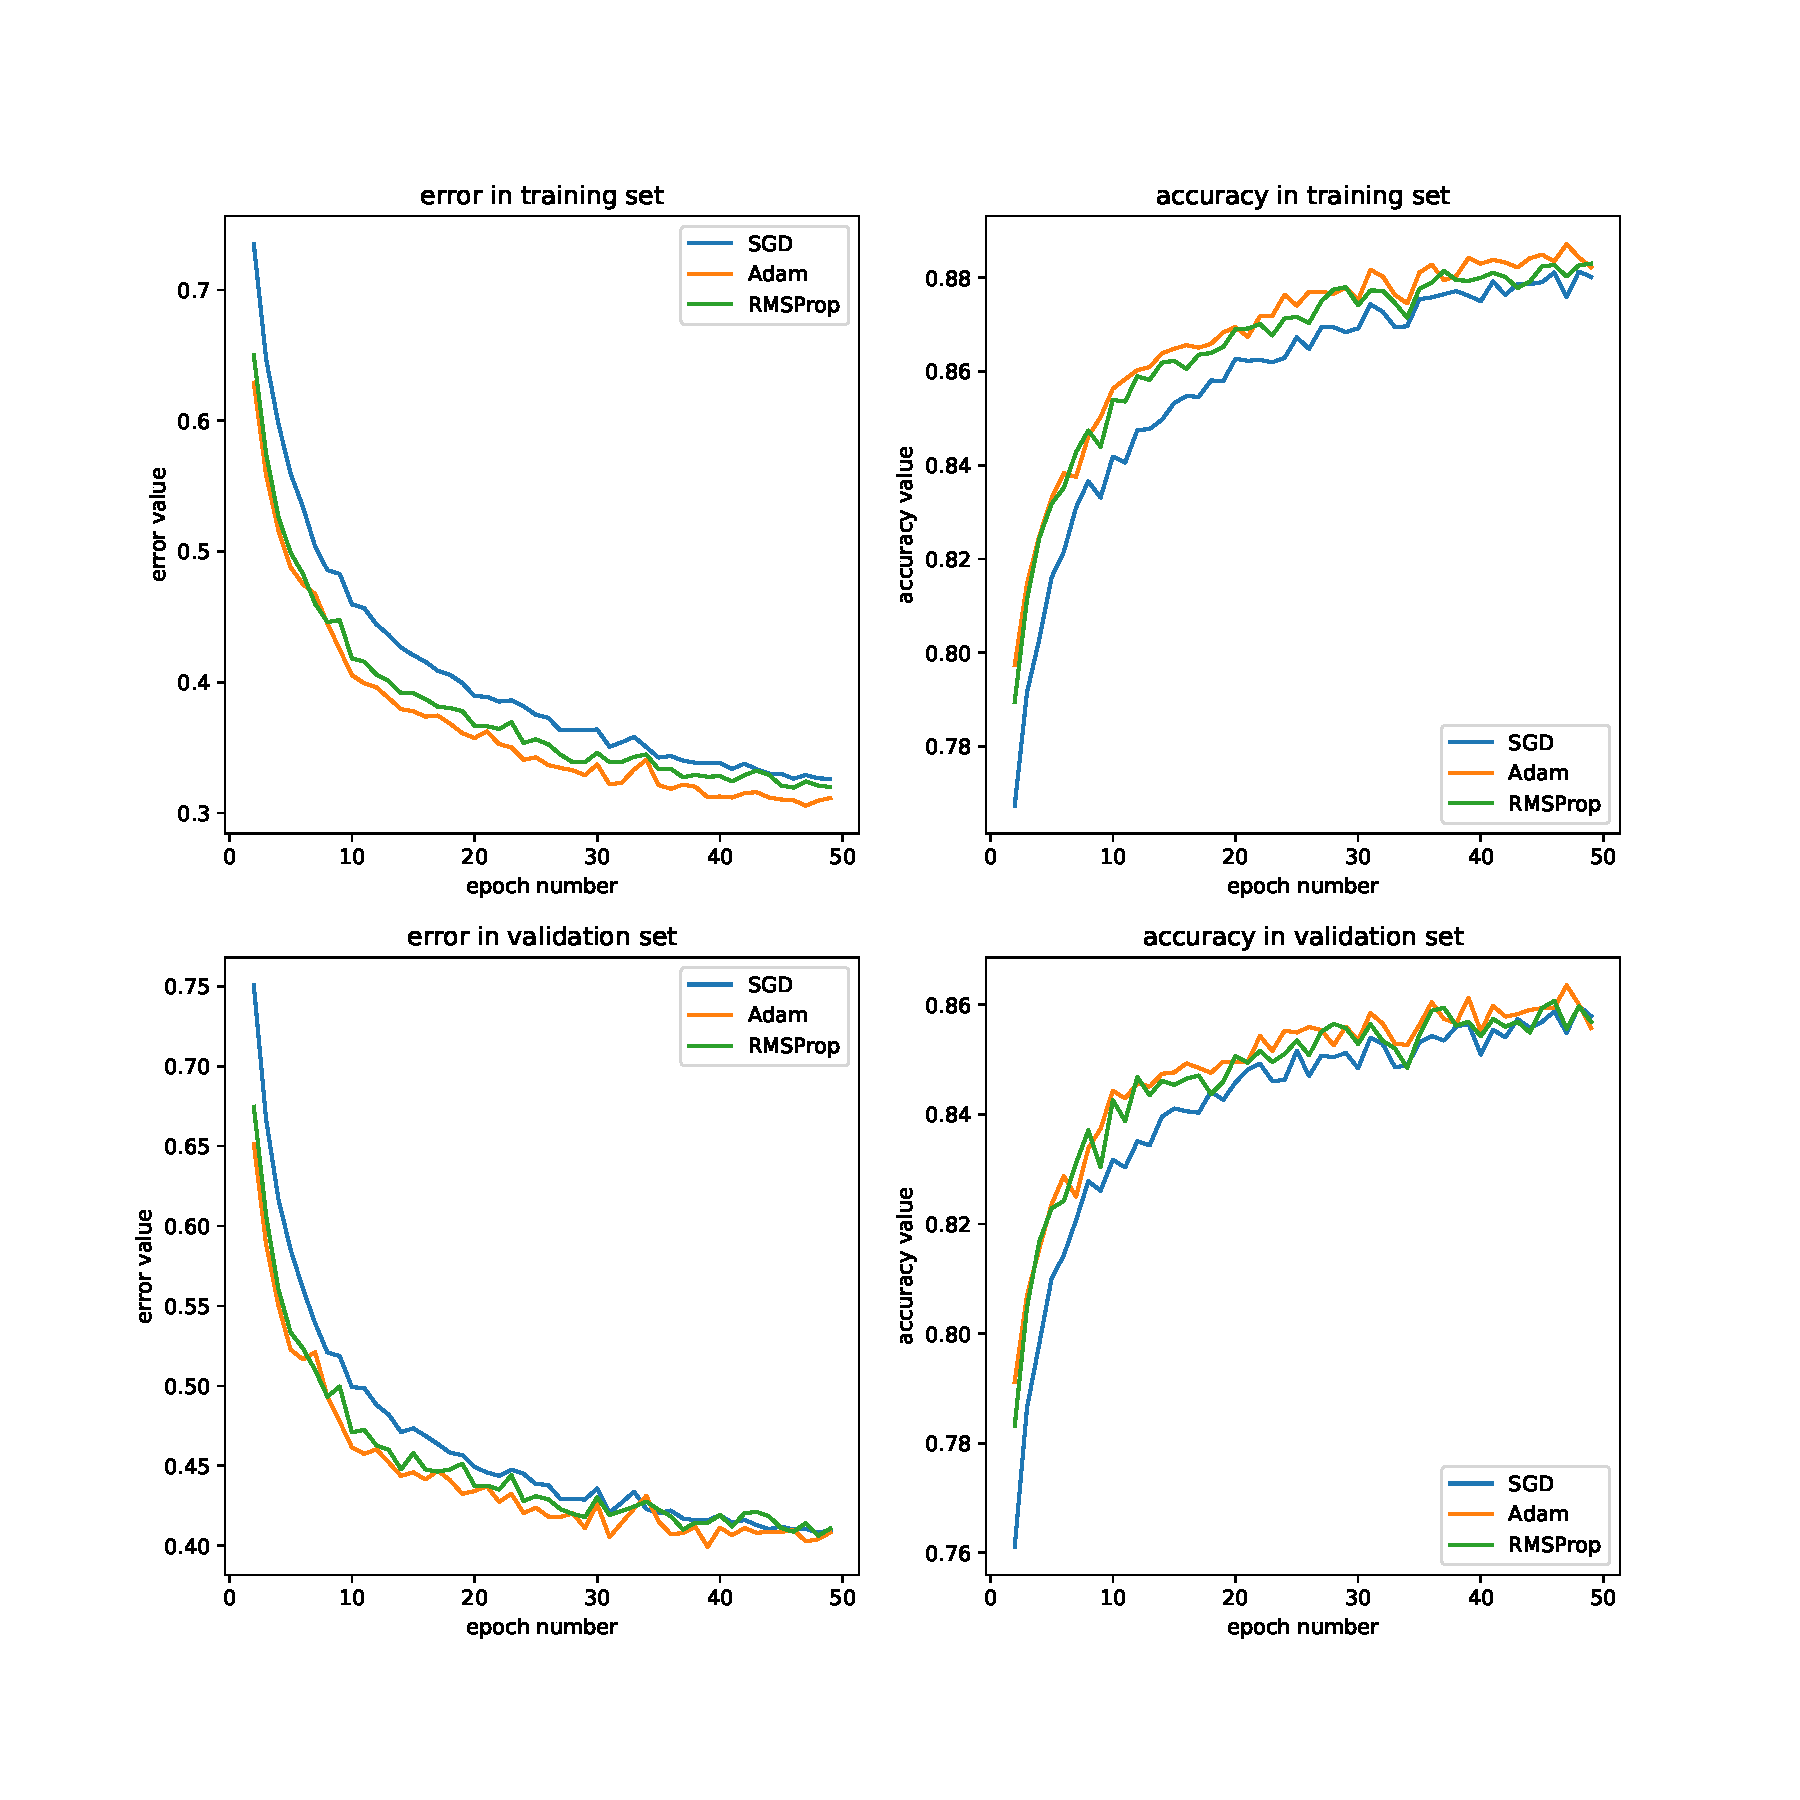
\includegraphics[width=\columnwidth]{fig/lr.pdf}}
\caption{Evaluate Adam, RMSProp and SGD}
\label{fig:lr}
\end{center}
\end{figure} 



%You should, in your own words, explain what the different learning rules do, and how they differ.  You should then present your experiments and results, comparing and contrasting stochastic gradient descent, RMSProp, and Adam.  As before concentrate on the ``what'' (remember give enough information so someone can reproduce your experiments), the ``why'' (why did you choose the experiments that you performed -- you may have been motivated by your earlier results, by the literature, or by a specific research question), and the interpretation of your results.

%In every section, you should present your results in a way that makes it easy for a reader to understand what they mean. You should facilitate comparisons either using graphs with multiple curves or (if appropriate, e.g. for accuracies) a results table. You need to avoid having too many figures, poorly labelled graphs, and graphs which should be comparable but which use different axis scales. A good presentation will enable the reader to compare trends in the same graph -- each graph should summarise the results relating to a particular research (sub)question.

%Your discussion should interpret the results, both in terms of summarising the outcomes of a particular experiment, and attempting to relate to the underlying models. A good report would have some analysis, resulting in an understanding of why particular results are observed, perhaps with reference to the literature. Use bibtex to organise your references -- in this case the references are in the file \verb+example-refs.bib+.  Here is a an example reference \citep{langley00}.  

\section{Batch normalisation}
Batch normalization \citep{DBLP:journals/corr/IoffeS15} is a method to normalize layer inputs.  The algorithm is described as Algorithm~\ref{alg:batchnorm}. In our experiments, we are expecting to see the features described in original paper. "Batch Normalization allows us to use much higher learning rates and be less careful about initialization. It also acts as a regularizer, in some cases eliminating the need for Dropout." \citep{DBLP:journals/corr/IoffeS15}
\subsection{Experiment result} 
The result of the experiment is shown in Figure~\ref{fig:batchnorm}.

\paragraph{Evaluating the feature of reducing overfit} Adding batch normalization layer did increases training speed and reduced overfit. From the graph, we can compare the curve of "Baseline without Dropout" and "BatchNorm without Dropout". We can see that "Baseline without Dropout" start to overfit ( we can tell from the increasing validation set error and decreasing validation set accuracy) after 30 epochs, while "BatchNorm without Dropout" didn't increase. 

The reason of this phenomenon is that regularizers are simply adding terms to error function and penalize some features of the weights that we don't want to see (for example, big weight values). Adding a batch normalization layer can do the job of regularizers in another way: it normalized the value so that there won't be extremely huge values anymore.


\paragraph{Comparing with Dropout} So we compared BatchNorm with dropout and without Dropout. We can have a look at Figure~\ref{fig:batchnorm} and compare the curve of "Baseline with Dropout" and "BatchNorm with Dropout". We can see that initially, the one with BatchNorm improves more quickly, but after 10 epoch, the one with BatchNorm slowed down. This might because having a extra layer can slow down the training process. %???%





\begin{figure}[tb]
\begin{center}
\centerline{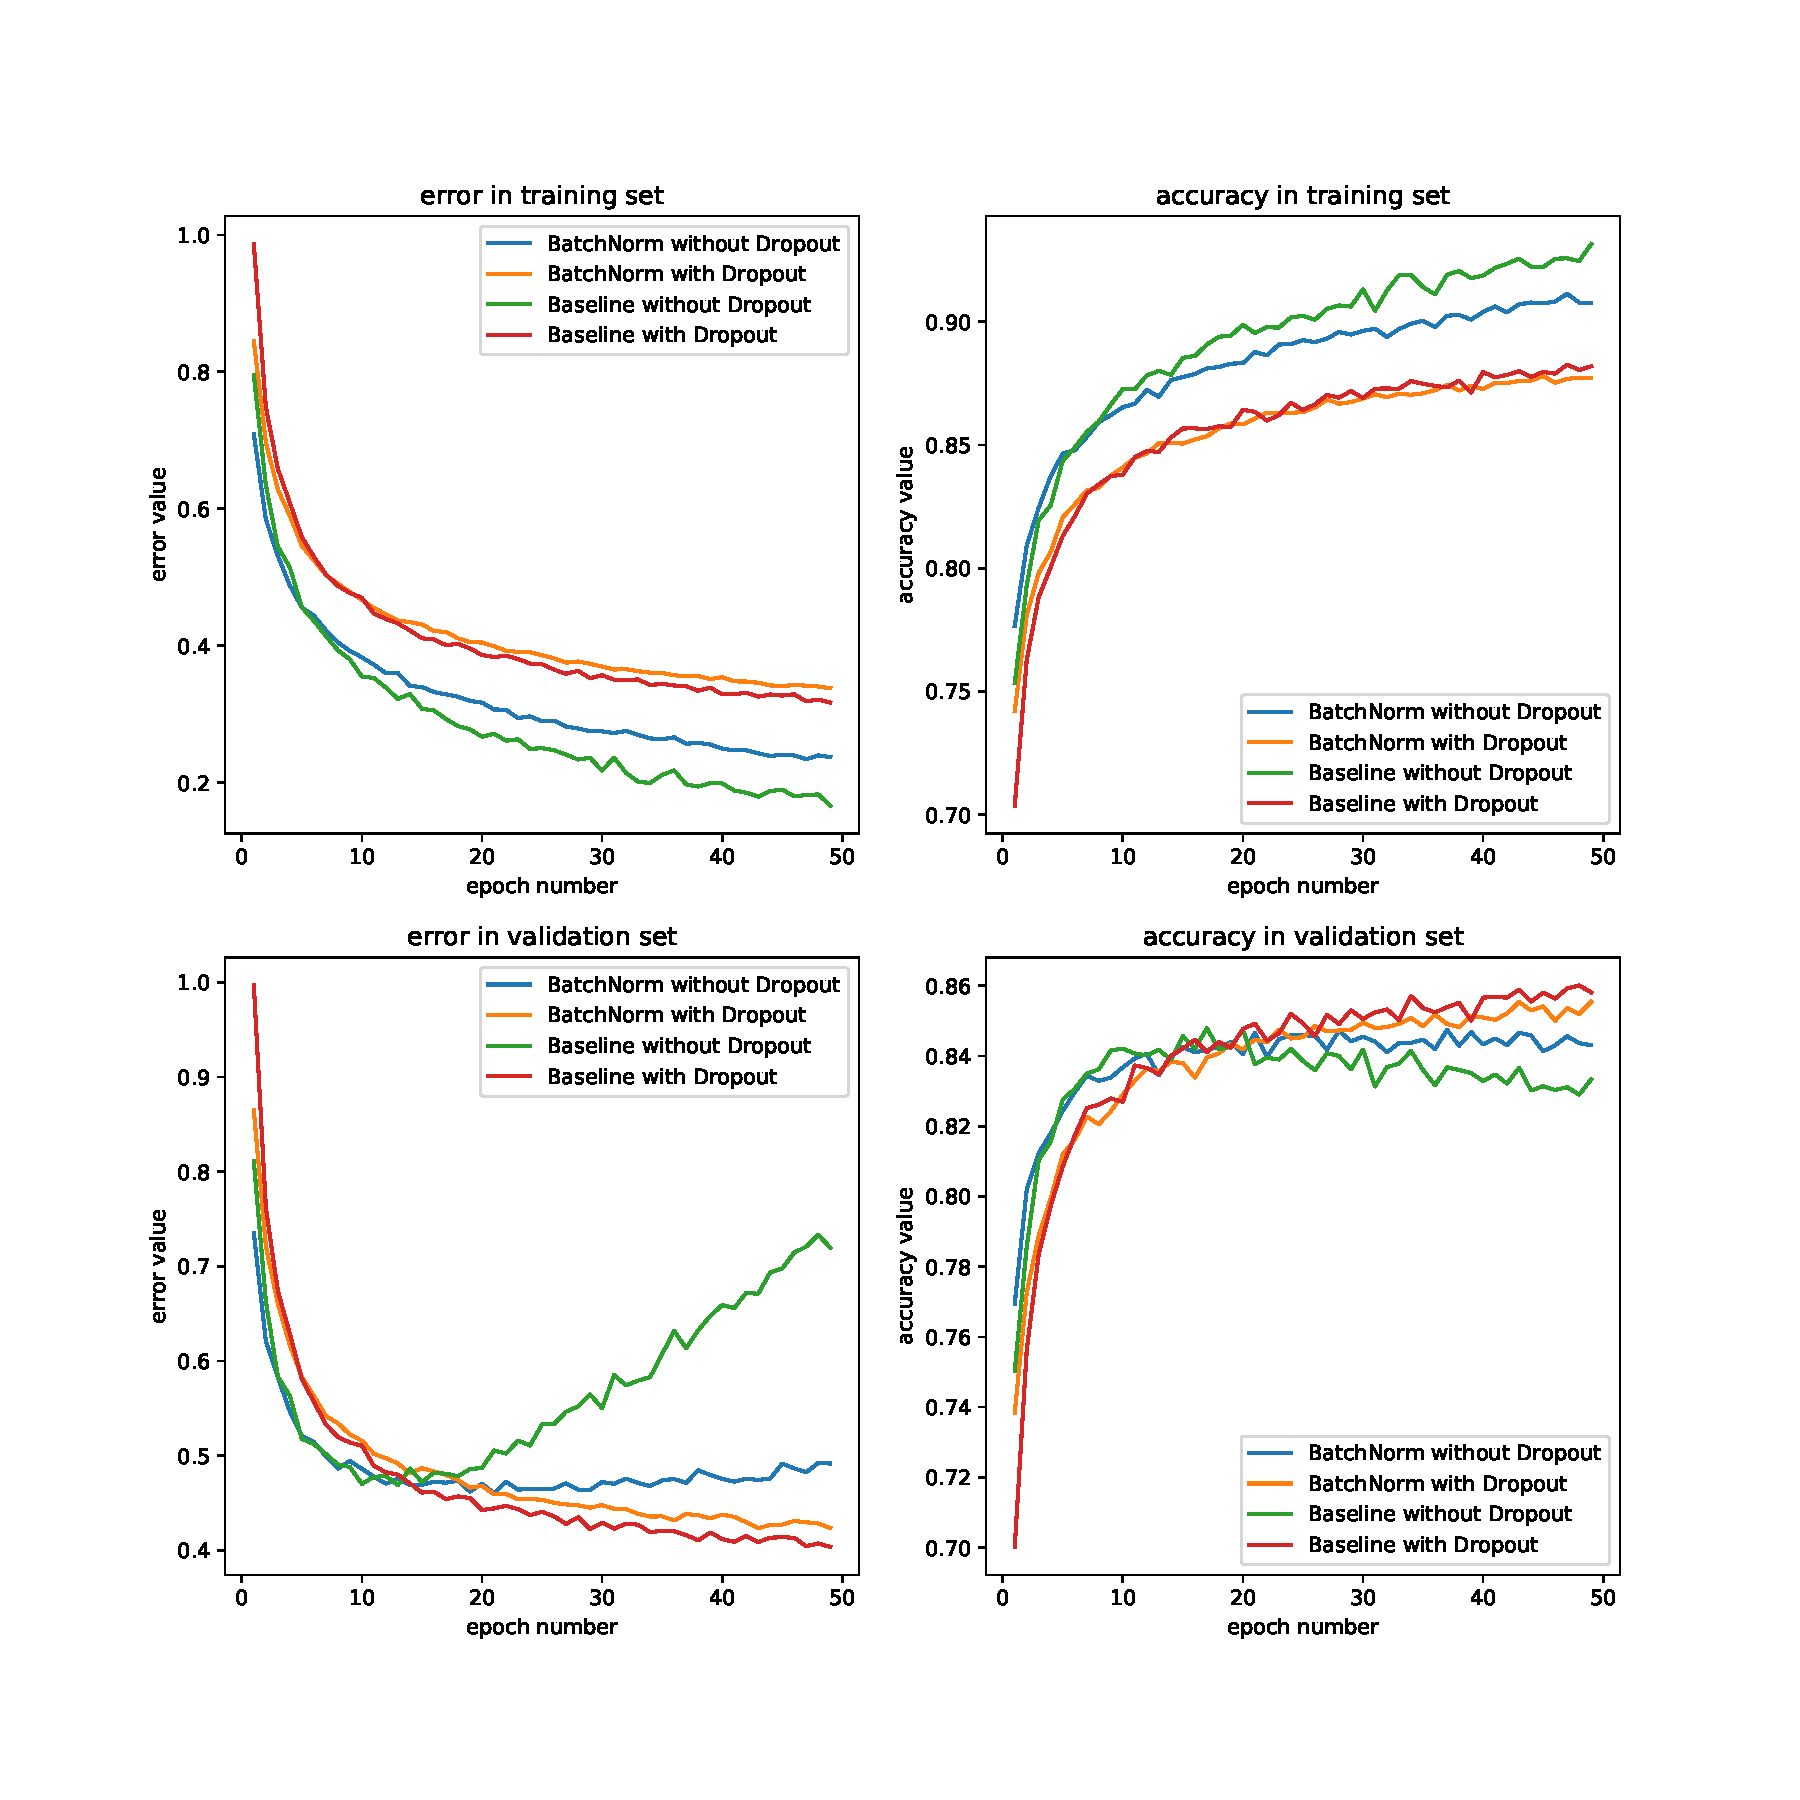
\includegraphics[width=\columnwidth]{fig/batchnorm.pdf}}
\caption{Evaluate batch norm.}
\label{fig:batchnorm}
\end{center}
\end{figure} 



\begin{algorithm}[ht]
\begin{algorithmic}
   \STATE {\bfseries Input:} Values of x over a mini-batch: $\mathcal{B} = {x_{1...m}}$
   \STATE {\bfseries Input:} Parameters to be learned: $\beta, \gamma$ 
   \STATE {\bfseries Output:} $y_i = BN_{\gamma,\beta}(x_i)$ 
   \STATE $\mu_{\mathcal{B}} \gets \frac{1}{m} \sum\limits_{i=1}^{m} x_i$
   \STATE $ \sigma^2_{\mathcal{B}} \gets \frac{1}{m} \sum\limits_{i=1}^{m} (x- \mu_B)^2 $
   \STATE $ \hat x_i \gets \frac{x_i-\mu_\mathcal{B}}{\sqrt{\sigma^2_{\mathcal{B}}+\epsilon}} $
   \STATE $ y_i  \gets \gamma \hat x_i + \beta \equiv  BN_{\gamma,\beta}(x_i) $
   
\end{algorithmic}
  \caption{Batch normalization }
  \label{alg:batchnorm}
\end{algorithm}





%In this section you should present batch normalisation,  supported using equations or algorithmic pseudocode.  Following this present your experiments, again remembering to include the ``what'', the ``why'', and the interpretation of results.

\section{Convolutional networks}
\subsection{Convolutional layer}

The idea of convolutional layer is to use shared filters to detect features and form feature maps. All the filters can be learned by back propagation when minimizing the error, but we still need to manually set filter size and number. The basic method is to apply filters to small windows of original picture and produce a feature map. Compared with the old method we use, which is simply flatten the picture into independent points, convolution layers can make use of the positional information and detect same feature in different place in the picture.

\paragraph{Implementing a convolution layer: a naive approach }
The most intuitive way to implement convolution layer is using for-loops. First loop over each example in mini-batch, for each example loop over filters. Then loop over sliding windows of filter size in original picture, and then multiply the windows matrix with filter matrix. This approach is quite easy to understand, but running quite slow in practice.


\paragraph{Implement a convolution layer: matrix manipulation. }
The for-loop version is quite slow and there is a better way to optimize it. The idea is, instead of use for-loop to move the sliding window and do dot product, we can expand the original matrix and gather all the possible locations that we can apply a filter to. This can be done by using im2col \citep{im2col} After we get the expanded matrix, we can do a dot product it. This optimized approach significantly boosted the performance. The original implementation takes 30 minutes for one epoch, while im2col version only needs 2 minutes.


\begin{figure}[tb]
\begin{center}
\centerline{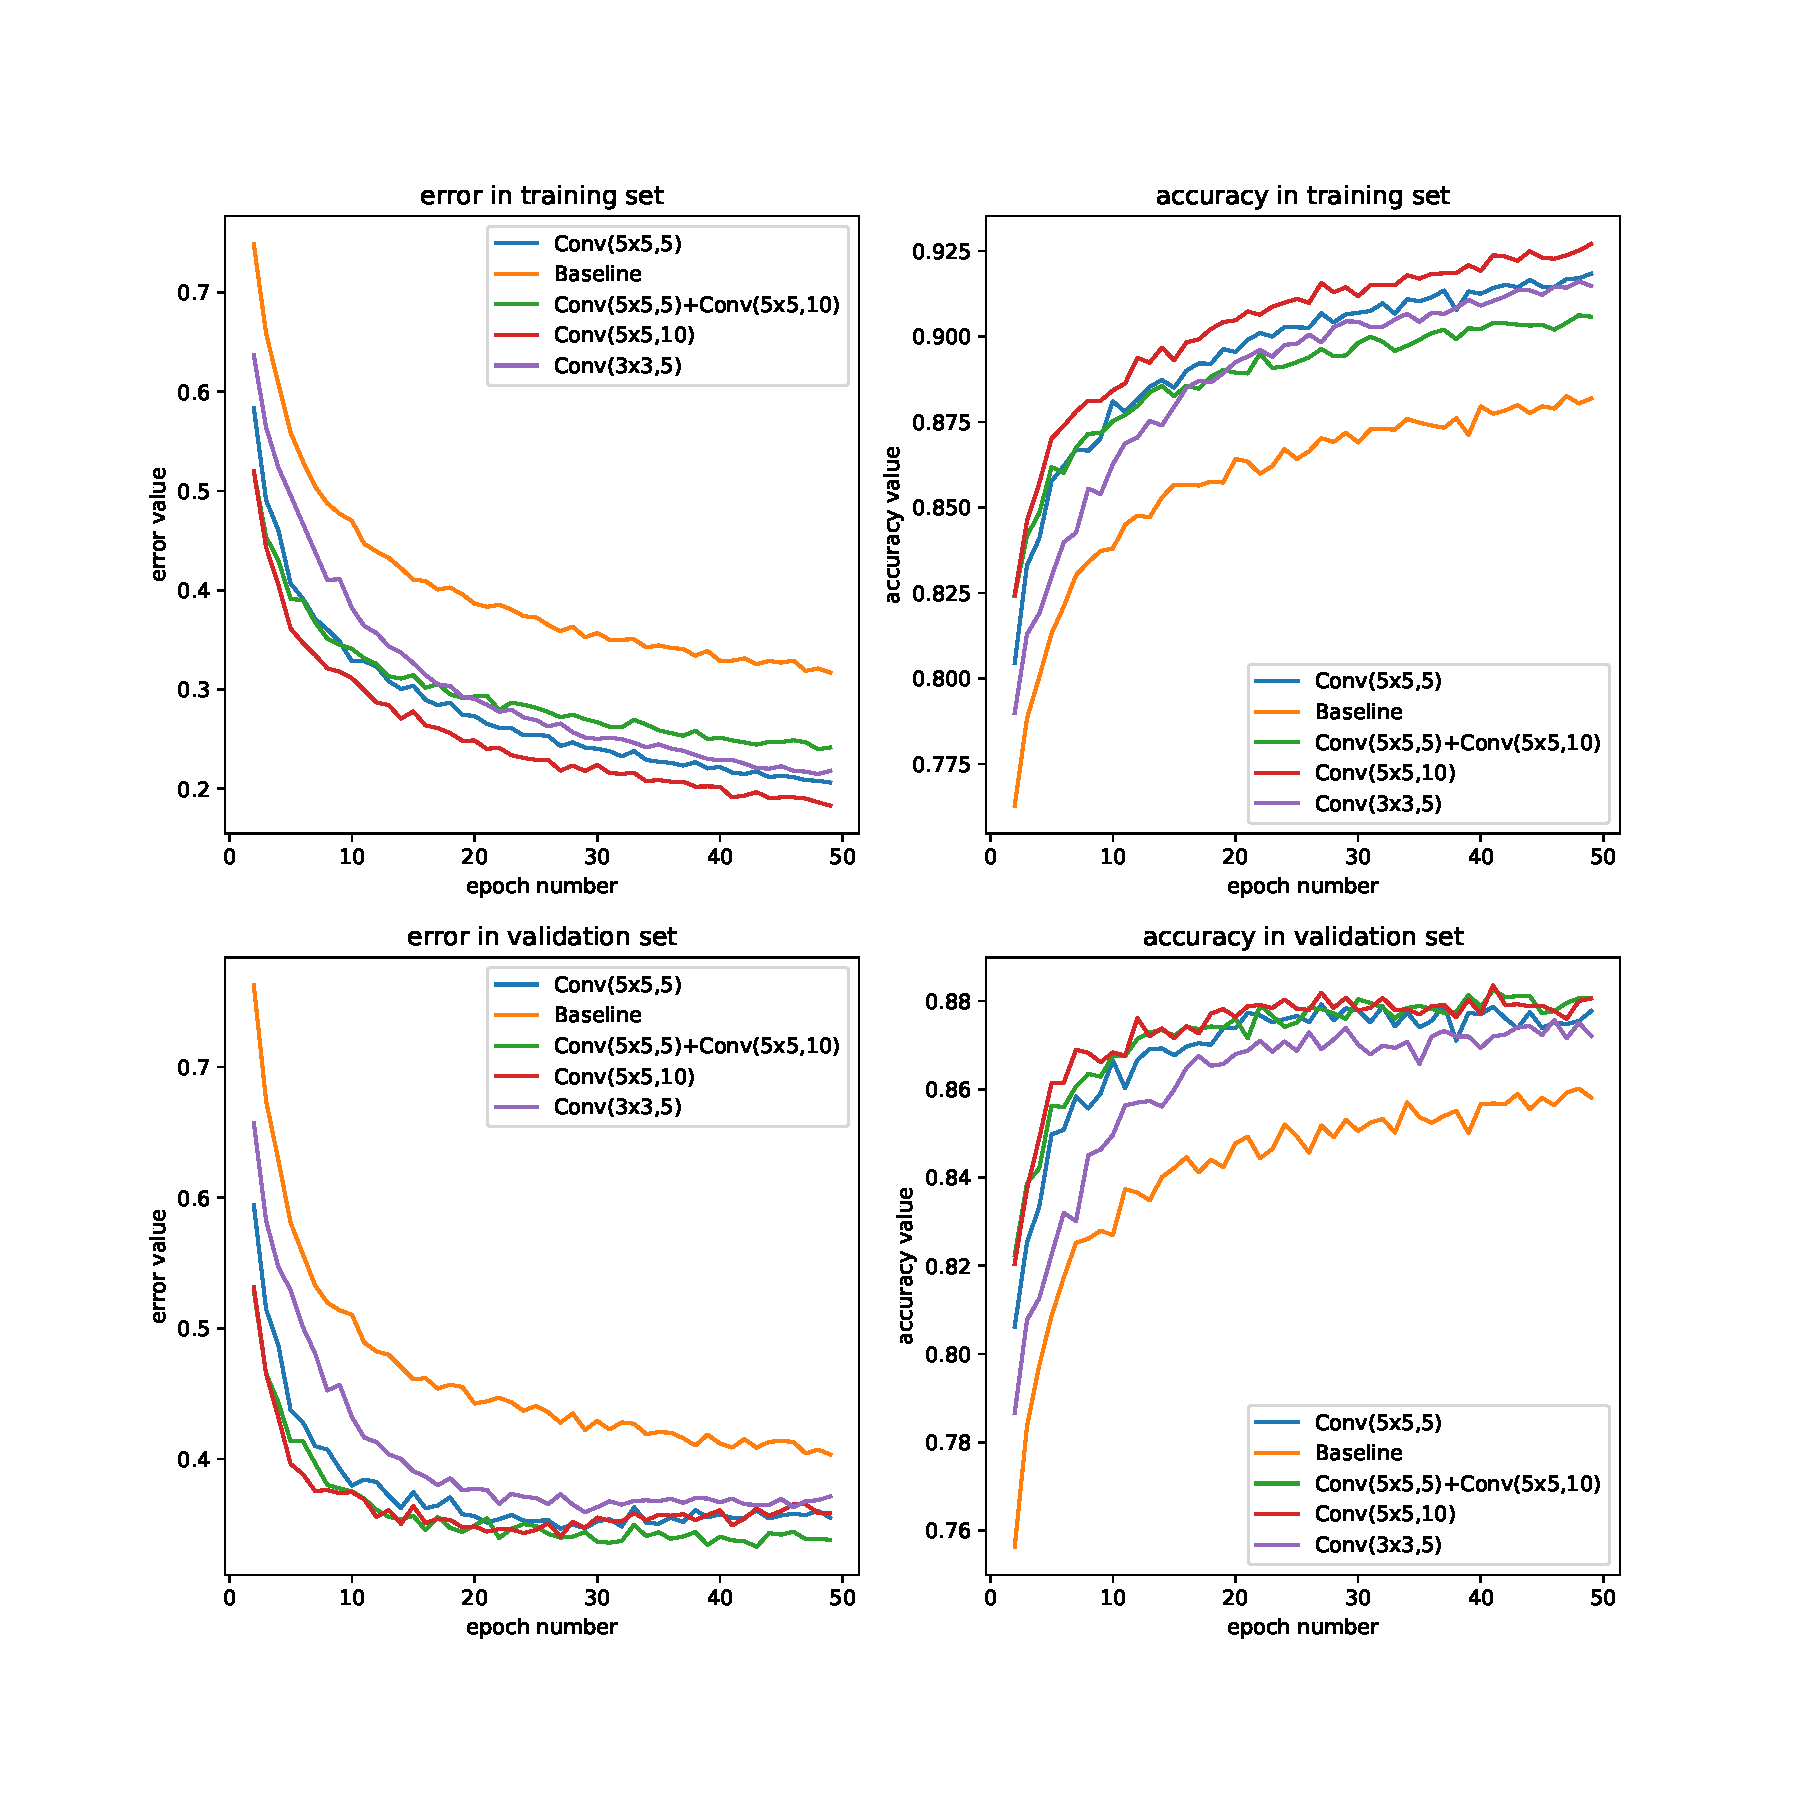
\includegraphics[width=\columnwidth]{fig/cnn.pdf}}
\caption{Evaluate batch norm.}
\label{fig:cnn}
\end{center}
\end{figure} 


\subsection{Maxpooling layer}
Maxpooling layer is basically shrinking the original matrix do use the max value of a sub matrix. This can reduce the size of feature map. The point of maxpooling is to shrink image size, and make significant features detected by convolutional layer less sparse. 
\paragraph{Implementing Maxpooling layer: naive approach}
Doing for-loop again is the most simple and direct method. Loop over all examples and loop over all channels, then get the sliding window matrix, replace it with the maximum value inside of it.

\paragraph{Implementing Maxpooling layer: matrix manipulation}
Similar to convolutional layer, this time we also need to expend the original matrix, but instead of doing dot product, we are going to apply max operation.

\subsection{Experiment}
The result is in Figure~\ref{fig:cnn}, and the test set accuracy is in Table~\ref{tab:cnn} . 
\paragraph{Comparing with baseline} 
We added 1 Convolutional Layer with 5 kernel number and 5x5 kernel size followed by an 2x2 2D Maxpooling Layer(curve "1 Conv Layer" in Figure~\ref{fig:cnn}) in front of the original baseline model. The network structure is as follows.

\begin{itemize}
	\item[->] Convoltional Layer (1 channel, 5 kernel, 5x5 feature map)
	\item[->] ELU Layer
	\item[->] 2D Maxpooling Layer ( 2 x 2 )
	\item[->] Baseline model
\end{itemize}

The improvement is quite significant. The reason I think is using convolutional layers did provided the following hidden layers with extra information which is helpful for classification, because convolutional layer can detect different features making use of the positional information using shared kernel. 

\paragraph{Difference between different number of convolutional layers. }
We compared models with different number of convolutional layers. Figure~\ref{fig:cnn} shows the curve. The curve "2 Conv Layer" is a model with an extra Convolutional layer and Maxpooling layer. The network structure is as follows. The reason I think is the second convolutional layer can help detect higher dimensional patterns as mentioned in \citep{Lecun98gradient-basedlearning}. First layer of convolutional network can detect low-level features like straight line, corners, the second convolutional layer can help form higher level features like cross, circle etc., because each window will contains more valid informations. For example, a 5x5 window in second convolutional layer contains extracted information(by maxpooling and kernel) of 14x14 space of original picture. With more higher dimensional features, the work of classification will become more easier, just like what we observed form the result.

\begin{itemize}
	\item[->] Convoltional Layer (1 channel, 5 kernel, 5x5 feature map)
	\item[->] ELU Layer
	\item[->] 2D Maxpooling Layer ( 2 x 2 )
	\item[->] Convolutional Layer (5 channel, 10 kernel, 5x5 feature map)
	\item[->] ELU Layer
	\item[->] 2D Maxpooling Layer ( 2 x 2 )
	\item[->] Baseline model
\end{itemize}

Comparing it with model "1 Conv Layer", we can see that the deeper one has better performance. As \citep{Lecun98gradient-basedlearning} described.

\paragraph{Different filter size}
We compared the performance of convolutional networks with different filter size. The curve "1 Conv Layer" has 5x5 filter size as mentioned above. The curve "1 Conv Layer 3x3" has 3x3 filter size in the first convolutional layer. The results turns out to be the one with bigger filter size performs better. I think tuning this parameter should based on specific dataset. As we have discussed above, this convolutional layer is trying to detect low level features of the picture. For EMNIST dataset, 3x3 window is too small to detect even low-level features.

\paragraph{Different filter number}
We also compared the performance of convolutional layers with different filter number. 



%In this section you should present your experiments with convolutional networks.  Explain the idea of convolutional layers and pooling layers, and briefly explain how you did the implementation.  There is no need to include chunks of code.  You should report the experiments you have undertaken, again remembering to include \emph{what} experiments you performed (include details of hyperparameters, etc.),  \emph{why} you performed them (what was the motivation for the experiments, what research questions are you exploring), and the interpretation and discussion of your results.

\begin{table}[tb]
\vskip 3mm
\begin{center}
\begin{small}
\begin{sc}
\begin{tabular}{lcccr}
\hline
\abovespace\belowspace
Model & Accuracy \\
\hline
\abovespace
2 Convolutional layer    	& 0.8680 	\\
1 Convolutional layer	 	& 0.8671 	\\
Baseline				  	& 0.8485 	\\

\hline
\end{tabular}
\end{sc}
\end{small}
\caption{Accuracy of models with different activation on test set}
\label{tab:cnn}
\end{center}
\vskip -3mm
\end{table}



% The results reported in the previous sections should be on the validation set.  You should finally report results on the EMNIST test set using what you judge to the be the best deep neural network (without convolutional layers) and the best convolutional network.  Again focus on what the experiments were (be precise), why you chose to do them (in particular, how did you choose the architectures/settings to use with the test set), and a discussion/interpretation of the results.


\section{Conclusions}
\label{sec:concl}
%You should draw conclusions from the experiments, related to the research questions outlined in the introduction (section~\ref{sec:intro}). You should state the conclusions clearly and concisely. It is good if the conclusion from one experiment influenced what you did in later experiments -- your aim is to learn from your experiments. Extra credit if you relate your findings to what has been reported in the literature.

%A good conclusions section would also include a further work discussion, building on work done so far, and referencing the literature where appropriate.

\bibliography{example-refs}

\end{document} 


% This document was modified from the file originally made available by
% Pat Langley and Andrea Danyluk for ICML-2K. This version was
% created by Lise Getoor and Tobias Scheffer, it was slightly modified  
% from the 2010 version by Thorsten Joachims & Johannes Fuernkranz, 
% slightly modified from the 2009 version by Kiri Wagstaff and 
% Sam Roweis's 2008 version, which is slightly modified from 
% Prasad Tadepalli's 2007 version which is a lightly 
% changed version of the previous year's version by Andrew Moore, 
% which was in turn edited from those of Kristian Kersting and 
% Codrina Lauth. Alex Smola contributed to the algorithmic style files.  
